\documentclass{beamer}

\usetheme{default}
\usecolortheme{rose}
\usepackage{hyperref}
\setbeamerfont{alerted text}{series=\itshape}
\newcommand{\ignore}[1]{}
\newcommand{\pr}{\mathbb{P}}
%\setbeamertemplate{footline}[frame number]
\addtobeamertemplate{navigation symbols}{}{%
    \usebeamerfont{footline}%
    \usebeamercolor[fg]{footline}%
    \hspace{1em}%
    \insertframenumber/\inserttotalframenumber
}

\title{Basic Probability}

% A subtitle is optional and this may be deleted
\subtitle{STAT-UB.0001 Statistics for Business Control}

\author{Ningshan Zhang}
% - Give the names in the same order as the appear in the paper.
% - Use the \inst{?} command only if the authors have different
%   affiliation.

\institute[New York University] % (optional, but mostly needed)
{
  IOMS Department\\
  nzhang@stern.nyu.edu
}
\date{July 5, 2018}
\AtBeginSubsection[]
{
  \begin{frame}<beamer>{Outline}
    \tableofcontents[currentsection,currentsubsection]
  \end{frame}
}

% Let's get started
\begin{document}

%-------------------
\begin{frame}
  \titlepage
\end{frame}



% Section and subsections will appear in the presentation overview
% and table of contents.


%-------------------
\begin{frame}{Review}
\begin{itemize}
\item Goal of this class: use a sample to make a statement about a population. 
\begin{itemize}
\item Representative sample and unbiased sample.
\item Sources of bias.
\end{itemize} 
\item Descriptive statistics: summarize data.
\begin{itemize}
\item Graphical summary. 
\item Numerical summary: mean, median, std, empirical rules.
\end{itemize}
\end{itemize}
\end{frame}



%-------------------
\begin{frame}{Probability}
Probability is the basic language of statistics.
\begin{center}
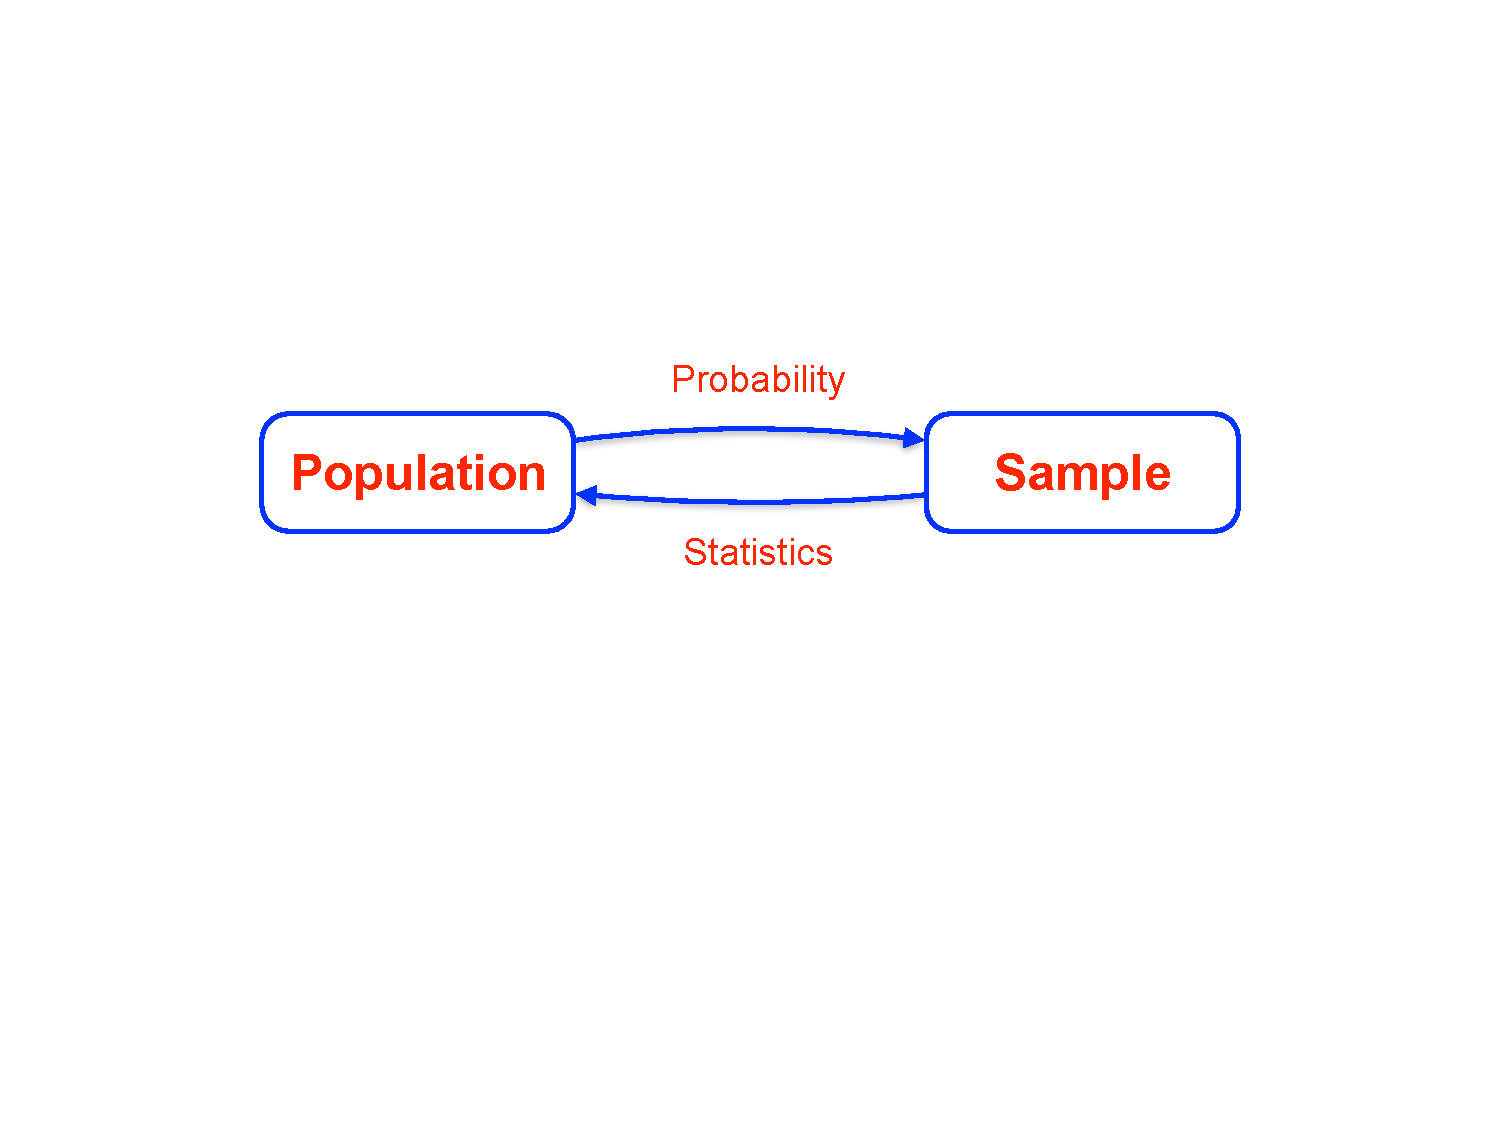
\includegraphics[width=0.8\textwidth]{figures/prob_and_stat.pdf}
\end{center}
\begin{block}{Probability vs Statistics}
\begin{itemize}
\item Probability: a fair coin is tossed 10 time; what is the probability of getting 8 heads?�
\item Statistics: a coin is tossed 10 times, showing 8 heads; is the coin fair?�
\end{itemize}
\end{block}
\end{frame}

%-------------------
\begin{frame}{Experiments, Sample Points, and Sample Spaces}
\begin{itemize}
\item Random experiment: the process of observation leading to an outcome that cannot be predicted with certainty.
\item Sample point: a possible outcome of an experiment. 
\item Sample space of experiments: the set of all sample points, denoted by $\Omega$, or $S$.
\end{itemize}
Example: flip a coin; roll a 6-sided dice.
\end{frame}


%-------------------
\begin{frame}{Probability}
Given a sample space, $\Omega=\{e_1,e_2,..e_n\}$. A probability 
$\pr$  is a function with two properties: 
\begin{itemize}
\item The probability of any sample point is nonnegative, 
$$\pr(e_i)\geq0.$$
\item The sum of probabilities is 1,
$$ \pr(e_1)+ .. + \pr(e_n)=1.$$
\end{itemize}
\end{frame}


%-------------------
\begin{frame}{Events}
Event is a set of sample points. Example:
\begin{itemize}
\item  A  fair die rolls odd.
\item A  fair die rolls 4 or higher.
\end{itemize}

\vspace{\stretch{0.5}}
Events are usually denoted by capital letters, e.g. $A$. If $A=\{f_1,\dots,f_m\}$, then
 $$\pr(A)=\pr(f_1) + \dots + \pr (f_m).$$
 
Example: Find the probabilities of the two events above.
\end{frame}



%-------------------
\begin{frame}{Compound Events: Union and Intersections}
$A$ and $B$ are two events.
\begin{itemize}
\item Union ($A \cup B$, ``$A$ or $B$''): event $A$ or event $B$ occurs, or both occur. 
\item Intersection ( $A \cap B$, ``$A$ and $B$''): event A and event B both occur.
\end{itemize}
\begin{center}
\begin{figure}\caption{Left: $A\cap B$. Right: $A\cup B$}
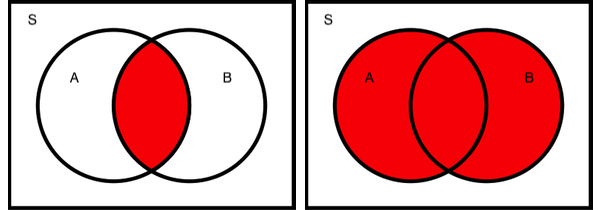
\includegraphics[width=0.6\textwidth]{figures/venn-intersection-union}
\end{figure}\end{center}
Example: 
 A = ``a die rolls odd'' and B = ``a die rolls 4 or higher''.
 What is $A\cup B$? What is $A\cap B$?
\end{frame}


%-------------------
\begin{frame}{Additive Rule}
Additive rule helps computing the probability of compound events:
$$ \pr(A\cup B) = \pr(A)+\pr(B) - \pr(A\cap B).$$
\vspace{\stretch{0.1}}

Example: 
 A = ``a die rolls odd'' and B = ``a die rolls 4 or higher''.

\begin{itemize}
\item $\pr(A)$
\item $\pr(B)$
\item $\pr(A\cap B)$
\item $\pr(A \cup B)$
\end{itemize}
\end{frame}

\begin{frame}{Mutually Exclusive Events}
\begin{itemize}
\item Events $A$ and $B$ are mutually exclusive (ME): $A$ and $B$  cannot occur together, $A\cap B=\emptyset$ (empty).
\item  Additive rule for \alert{mutually exclusive} events:
$$\pr(A\cup B)=\pr(A)+\pr(B).$$
\end{itemize}
\vspace{\stretch{0.1}}

Example:
\begin{itemize}
\item ``a die rolls 3'' and ``a die rolls 4'' 
\item ``a die rolls odd'' and ``a die rolls 4 or higher'' 
\end{itemize}
\end{frame}


%-------------------
\begin{frame}{Complementary Event}
\begin{itemize}
\item Complement of event $A$ ($A^c$, $\bar A$, ``not $A$'' ):  event $A$ does not occur.
\item $A$ and $A^c$ are mutually exclusive events. 
\item  Complement rule: 
$$ \pr(A^c) = 1 - \pr(A).$$
\end{itemize}
\vspace{\stretch{0.2}}

Example:  Suppose you flip a fair coin five times. What is the probability of getting at least one head?
\ignore{
 A=``A fair coin shows 4 heads or less out of 5 tosses''.
\begin{itemize}
\item $\pr(A)$
\item $\pr(A^c)$
\end{itemize}
}
\end{frame}

%-------------------
\begin{frame}{Interpretations of Probability}
\begin{itemize}
\item Long-run relative frequency: when an  experiment is repeated $n$  times ($n$ is large),
$$\pr(A) \approx (\text{no. of times }A\text{ occured})/n.$$
\item In daily conversation, the probability is a statement about how much you believe something to be true.
\begin{itemize}
\item Example: there is 10\% probability of rain tomorrow.
\item It's different from the way we use probability in this class.
\end{itemize}
\end{itemize}
\end{frame}


%-------------------
\begin{frame}{Conditional Probability}
$\pr(A \mid B)$:  the probability of event $A$, given that event $B$ occurred. It is formally defined as 
$$\pr(A\mid B) = \frac{\pr(A \cap B)}{\pr(B)}.$$

Other interpretations:
\begin{itemize}
\item If I know the sample point is in $B$, what is the chance it is also in $A$.
\item Equivalently, among all the sample points in $B$, what is the proportion of sample points that are also in $ A$.
\end{itemize}

\end{frame}


%-------------------
\begin{frame}{Multiplicative Rule}
Multiplicative rule helps to compute the prob. of interactions:
$$\pr(A \cap B) = \pr(B) \pr(A\mid B) = \pr(A)\pr(B \mid A).$$

Example:  Box A contains 8 red and 2 green balls; box B contains 15 red and 30 green balls. Flip a fair coin, and select a ball from box A if  heads, or from box B if  tails. Find
\begin{itemize}
\item $\pr(\text{red}\mid\text{heads})$
\item $\pr(\text{red}\mid\text{tails})$
\item $\pr(\text{red and heads})$
\item $\pr(\text{red and tails})$
\item $\pr(\text{red})$
\end{itemize}
\end{frame}

\begin{frame}{Summary}
\begin{itemize}
\item Random experiment, sample point, sample space
\item Probability
\item Events, union and intersection, mutually exclusive events, complementary event
\item Additive rule
\item Conditional probability, multiplicative rule
\end{itemize}
\end{frame}

\ignore{
%-------------------
\begin{frame}{}
\begin{itemize}
\item 
\end{itemize}
\end{frame}
}



\end{document}


